\documentclass[../main.tex]{subfiles}


\begin{document}

%%%%%%%%%%%%%%%%%%%%%%%%%%%%%%%%%%%%%%%%%%%%%%%%%%%%%%%%%%%%%%%%%%%%%%%%%%%%%%%%%%%%%%%%%%%%%%%%%%%%%%%%%
\section{Metrické prostory}
%%%%%%%%%%%%%%%%%%%%%%%%%%%%%%%%%%%%%%%%%%%%%%%%%%%%%%%%%%%%%%%%%%%%%%%%%%%%%%%%%%%%%%%%%%%%%%%%%%%%%%%%%
\subsection{Definice metrického prostoru}
\hspace{1.2mm}
Metrický prostor : Nechť $X$ je množina,  $d: X \times X \rightarrow \mathbb{R}$ funkce t. ž. platí:

\begin{itemize}
\item{$\forall x,y \in X : d(x,y) \geq 0, d(x,y) \iff x = y$ }
\item{$\forall x,y \in X : d(x,y) = d(y,x)$}
\item{$\forall x,y \in X : d(x,z) \leq d(x,y) + d(y,z)$ (trojúhelníková nerovnost)}
\end{itemize}
pak $(X,d)$ je metrický prostor.

\noindent
\hspace{1.2mm}
Příklady:
\begin{align*} 
    (\mathbb{R}, |x-y|) &,
    (\mathbb{C},|x-y|) &,
    (G,d) &, \textrm(G je orientovaný souvislý graf,) d \textrm{je délka nejdelší cesty}\\
\end{align*}

\hspace{1.2mm}
Pozor: trojúhelníková nerovnost v $(\mathbb{C}, |x-y|)$ není tak triviální jako v $\mathbb{R}$.
%%%%%%%%%%%%%%%%%%%%%%%%%%%%%%%%%%%%%%%%%%%%%%%%%%%%%%%%%%%%%%%%%%%%%%%%%%%%%%%%%%%%%%%%%%%%%%%%%%%%%%%%%

\subsection{Euklidovský prostor $\mathbb{E}_n$}
\hspace{1.2mm}
Definujeme jako $(\mathbb{R}^n,d)$, kde $d$:
\[d((x_1,...,x_n),(y_1,...,y_n)) = \sqrt{\sum_i(x_i-y_i)^2}\]

Pro nás zvlášť důležitý, známy v podobě vektorového prostoru $\textbf{V}_n$ se skalárním součinem $\textbf{u}v$ a normou
$||\textbf{u}|| = \sqrt{\textbf{uu}}$ a vzdáleností $||\textbf{u}-\textbf{v}||$
\noindent

%%%%%%%%%%%%%%%%%%%%%%%%%%%%%%%%%%%%%%%%%%%%%%%%%%%%%%%%%%%%%%%%%%%%%%%%%%%%%%%%%%%%%%%%%%%%%%%%%%%%%%%%%
\subsection{Diskrétní prostor}
\hspace{1.2mm}
Definujeme jako $(X,d)$, kde $d(x,y) = 1$ pro $x \neq y$
\noindent

%%%%%%%%%%%%%%%%%%%%%%%%%%%%%%%%%%%%%%%%%%%%%%%%%%%%%%%%%%%%%%%%%%%%%%%%%%%%%%%%%%%%%%%%%%%%%%%%%%%%%%%%%
\subsection{Podprostor}
\hspace{1.2mm}
Buď $(X, d)$ metrický prostor. Pak $(Y, d')$ je podprostor, kde $Y \subseteq X$ a $d'(x,y) = d(x,y)$.

%%%%%%%%%%%%%%%%%%%%%%%%%%%%%%%%%%%%%%%%%%%%%%%%%%%%%%%%%%%%%%%%%%%%%%%%%%%%%%%%%%%%%%%%%%%%%%%%%%%%%%%%%
\subsection{Spojité zobrazení}
\hspace{1.2mm}
$f: (X,d) \to (Y, d')$ je spojité zobrazení, pokud
\[ \forall x \in X, \forall \epsilon > 0 \exists \delta > 0:
d(x,y) < \delta \Rightarrow d'(f(x), f(x)) < \epsilon \]

\subsection{Triviality}
\subsubsection{Identické zobrazení}

\hspace{1.2mm}
\[ (X,d) \to (X,d) \]

\subsubsection{Vložení podprostoru}

\hspace{1.2mm}
\[ j = (x \mapsto x): (Y,d') \to (X,d) \]

\subsubsection{Složení spojitých zobrazení je spojité}

\hspace{1.2mm}
Pokud jsou $f: (X,d) \to (Y, d')$ a $g: (Y,d') \to (Z, d'')$ spojité, pak i
\[ g \circ f: (X,d) \to (Z,d'') \] je spojité.

%%%%%%%%%%%%%%%%%%%%%%%%%%%%%%%%%%%%%%%%%%%%%%%%%%%%%%%%%%%%%%%%%%%%%%%%%%%%%%%%%%%%%%%%%%%%%%%%%%%%%%%%%
\subsection{Věta o konvergenci}
\hspace{1.2mm}
Zobrazení $f: (X_1,d_1) \rightarrow (X_2,d_2)$ je spojité právě když pro každou konvergentní $(x_n)_n v (X_1,d_1)$ 
posloupnost $(f(x_n))_n$ konverguje v $(X_2,d_2)$ a platí $\lim_n f(x_n) = f(\lim_n x_n)$.

\noindent
\hspace{1.2mm}
\textbf{Důkaz:}
Buď $f$ spojitá a nechť $\lim_nx_n = x$. Pro $\epsilon > 0$ svolme ze spojitosti $\delta > 0$
tak aby $d_2(f(y),f(x)) <\epsilon$ pro $d_1(x,y) < \delta$.
Podle definice konvergence posloupnosti existuje $n_0$ takové, že pro $n\geq n_0$ je $d_1(x_n,x) < \delta$. Tedy je-li $n \leq n_0$
máme $d_2(f(x_n),f(x)) < \epsilon$ a potom $\lim_n f(x_n) = f(\lim_n x_n)$.


%%%%%%%%%%%%%%%%%%%%%%%%%%%%%%%%%%%%%%%%%%%%%%%%%%%%%%%%%%%%%%%%%%%%%%%%%%%%%%%%%%%%%%%%%%%%%%%%%%%%%%%%%
\subsection{Okolí}
\hspace{1.2mm}
$\Omega (x,\epsilon) = \{ y | d(x,y) < \epsilon \}$

\vspace{5mm}

\noindent
\hspace{1.2mm}
\textbf{Užití:}
$"\textrm{U je okolí } x" \equiv \exists \epsilon > 0, \Omega (x,\epsilon) \subseteq U $

%%%%%%%%%%%%%%%%%%%%%%%%%%%%%%%%%%%%%%%%%%%%%%%%%%%%%%%%%%%%%%%%%%%%%%%%%%%%%%%%%%%%%%%%%%%%%%%%%%%%%%%%%
\subsection{Otevřená a uzavřená množina}
\hspace{1.2mm}
$U \subseteq (X,d)$ je \textbf{otevřená}, pokud je okolím \textit{každého} svého bodu.

\vspace{5mm}

\noindent
\hspace{1.2mm}
$V \subseteq (X,d)$ je \textbf{uzavřená}, pokud $\forall (x_n)_n \subseteq A$ je konvergentní
v $X$ je $\lim_n x_n$ v $A$.

%%%%%%%%%%%%%%%%%%%%%%%%%%%%%%%%%%%%%%%%%%%%%%%%%%%%%%%%%%%%%%%%%%%%%%%%%%%%%%%%%%%%%%%%%%%%%%%%%%%%%%%%%
\subsection{Uzávěr}
\hspace{1.2mm}
\textbf{Uzávěr} $A$ je $\overline{A} = \{ x | d(x,A) = 0 \}$

%%%%%%%%%%%%%%%%%%%%%%%%%%%%%%%%%%%%%%%%%%%%%%%%%%%%%%%%%%%%%%%%%%%%%%%%%%%%%%%%%%%%%%%%%%%%%%%%%%%%%%%%%
\subsection{Vlastnosti zobrazení mezi metrickými prostory}
\hspace{1.2mm}
Buďte $(X_1, d_1)$ a $(X_2, d_2)$ metrické prostory a buď zobrazení $f: X_1 \to X_2$. Následující
jsou potom ekvivalentní:
\begin{enumerate}
    \item $f$ je spojité.
    \item $\forall x \in X_1$ a $\forall$ okolí $V$ bodu $f(x)$ existuje okolí $U$ bodu $x$ takové, že
        $f[U] \subseteq V$.
    \item $\forall$ otevřenou $U$ v $X_2$ je vzor $f^{-1}[U]$ otevřený v $X_1$.
    \item $\forall$ uzavřenou $A$ v $X_2$ je vzor $f^{-1}[U]$ uzavřený v $X_1$.
    \item $\forall A \subseteq X_1$ je $f[\overline{A}] \subseteq \overline{f[A]}$
\end{enumerate}


%%%%%%%%%%%%%%%%%%%%%%%%%%%%%%%%%%%%%%%%%%%%%%%%%%%%%%%%%%%%%%%%%%%%%%%%%%%%%%%%%%%%%%%%%%%%%%%%%%%%%%%%%
\subsection{Silně ekvivalentní metriky}
\hspace{1.2mm}
Buďte $d_1, d_2$ metriky. $d_1$ a $d_2$ na téže jsou silně ekvivalentní, pokud
\[\exists \alpha , \beta > 0: \alpha d_1(x,y) \leq d_2(x,y) \leq \beta d_1(x,y)\]

%%%%%%%%%%%%%%%%%%%%%%%%%%%%%%%%%%%%%%%%%%%%%%%%%%%%%%%%%%%%%%%%%%%%%%%%%%%%%%%%%%%%%%%%%%%%%%%%%%%%%%%%%
\subsection{Vzory a obrazy}
\hspace{1.2mm}
$f: X \rightarrow Y, A \subseteq X, B \subseteq Y$
%%%%%%%%%%%%%%%%%%%%%%%%%%%%%%%%%%%%%%%%%%%%%%%%%%%%%%%%%%%%%%%%%%%%%%%%%%%%%%%%%%%%%%%%%%%%%%%%%%%%%%%%%
\subsubsection{Obraz}
\hspace{1.2mm}
\underline{Obraz} podmnožiny $A\subseteq X$ v $Y$:
\[f[A] = \{f(x) | x \in A\}\]

%%%%%%%%%%%%%%%%%%%%%%%%%%%%%%%%%%%%%%%%%%%%%%%%%%%%%%%%%%%%%%%%%%%%%%%%%%%%%%%%%%%%%%%%%%%%%%%%%%%%%%%%%
\subsubsection{Vzor}
\hspace{1.2mm}
\underline{Vzor} podmnožiny $B\subseteq Y$ v $X$:
\[f^{-1}[B] = \{x | f(x) \in B\}\]
\[X \underset{f^{-1}[-]}{\stackrel{f[-]}{\rightleftarrows}} Y\]
\hspace{1.2mm}
Platí:
\[f[A] \subseteq B \equiv A \subseteq f^{-1}[B],\]
\[f[f^{-1}[B]] \subseteq B  ...  f^{-1}[f[A]] \supseteq A\]

\noindent
\hspace{1.2mm}
\textbf{Pozor:} $f^{-1}$ má dvá významy:
\begin{itemize}
    \item inverze $f^{-1}:Y \rightarrow X$, nemusí existovat
    \item část v symbolu $f^{-1}[-]$, má smysl vždy
 
\end{itemize}
\noindent

%%%%%%%%%%%%%%%%%%%%%%%%%%%%%%%%%%%%%%%%%%%%%%%%%%%%%%%%%%%%%%%%%%%%%%%%%%%%%%%%%%%%%%%%%%%%%%%%%%%%%%%%%
\subsection{Reálná funkce o $n$ proměnných}
\hspace{1.2mm}
\[f: D \rightarrow \mathbb{R}, D \subseteq \mathbb{E}_n\]

\noindent
\hspace{1.2mm}
Podobně jako ve funkcích jedné proměnné se nemůžeme omezit na případy, kdy definiční obor je celý prostor $\mathbb{E}_n$. V 
Případě funkcí jedné proměnné byly definiční obory obvykle intervaly nebo jednoduchá sjednocení intervalů. Tady budou definiční
obory $D$ složitější, často (ale né vždy) otevřené množiny v $\mathbb{E}_n$.

O $D$ se často mluví jako o oblasti na níž je funkce definovaná. To není termín (ve specifických kontextech slovo "oblast" termín 
je, tady ne).

%%%%%%%%%%%%%%%%%%%%%%%%%%%%%%%%%%%%%%%%%%%%%%%%%%%%%%%%%%%%%%%%%%%%%%%%%%%%%%%%%%%%%%%%%%%%%%%%%%%%%%%%%
\subsection{Součiny}
\hspace{1.2mm}
Pro $(X_1,d_i), i = 1,...,n$ definujeme na kartézskem součinu $\prod^n_{i=1}X_i$ metriku
\[d((x_1,...,x_n),(y_1,...,y_n)) = \max_i d_i(x_i,y_i)\]
Získaný
\[\left(\prod^n_{i=1}X_i,d_i\right) = \prod^n_{i=1}(X_i,d_i)\]
se nazývá součin prostorů $(X_i, d_i)$. Píše se též 
\[(X_1,d_1) \times \cdot \cdot \cdot \times (X_n,d_n).\]

%%%%%%%%%%%%%%%%%%%%%%%%%%%%%%%%%%%%%%%%%%%%%%%%%%%%%%%%%%%%%%%%%%%%%%%%%%%%%%%%%%%%%%%%%%%%%%%%%%%%%%%%%
\subsection{Věta o spojitých zobrazeních}
\begin{enumerate}
\item Projekce $p_j = ((x_i)_i \mapsto x_j) : \prod^n_{i=1}(X_i,d_i) \rightarrow (X_j,d_j)$ jsou spojitá zobrazení.

\item Buďte $f_j:(Y,d') \rightarrow (X_j,d_j)$ libovolná spojitá zobrazení. Potom jednoznačně určené zobrazení 
$f:(Y,d') \rightarrow \prod^n_{i=1}(X_i,d_i)$ splňujíci $p_j \circ f = f_j$, totiž zobrazení definované předpisem
$f(y) = (f_1(y),...,f_n(y))$, je spojité.
\end{enumerate}
Jak to vypadá:
\begin{center}
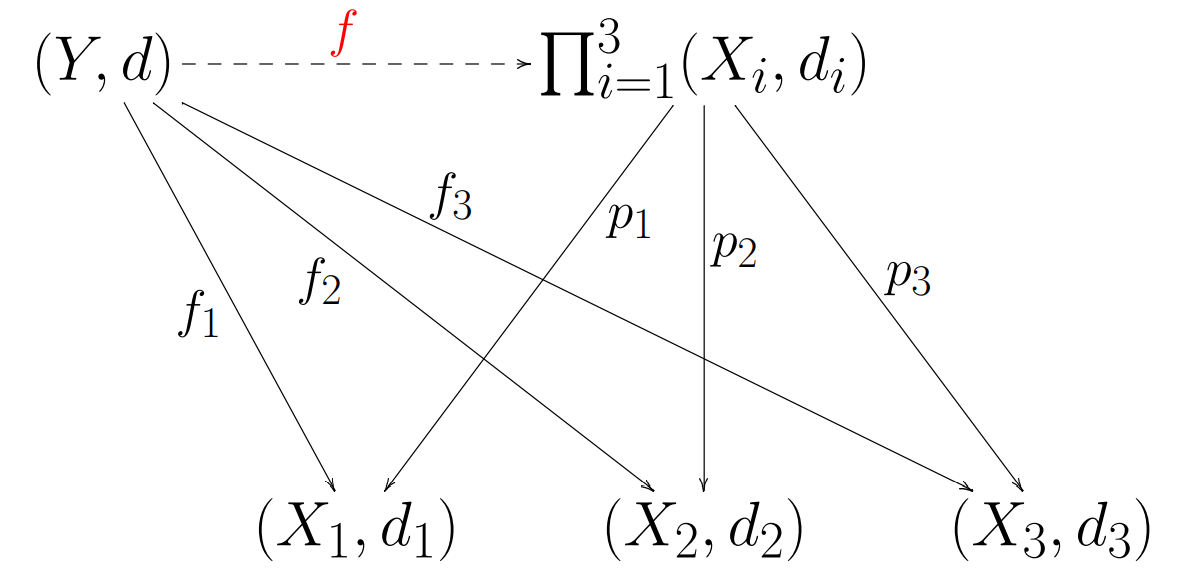
\includegraphics[width=9cm,height=4.8cm]{ipkm.png}
\end{center}
Existuje přesně jedno $f$ takové, že 
\[p_i \circ f = f_i\]
a je spojité.

\end{document}